\documentclass[dvipsnames, tikz]{standalone}
\usepackage{amsmath}
\usepackage{arevmath}
\usepackage{xcolor}
\usepackage{tikz}
\usetikzlibrary{calc}
\usetikzlibrary{decorations.pathreplacing,calligraphy,3d}
\usetikzlibrary{matrix,shapes,fit,backgrounds}

\tikzset{%
	orange/.pic={
		\fill [BurntOrange!80] (0,0) circle [radius=1];
		\fill [BurntOrange] (0,0) -- (45:1) arc (45:-135:1) -- cycle;
		\fill [BurntOrange, shift={(0,3/4)}] coordinate (@)
		ellipse [x radius=1/4, y radius=1/8];
		\begin{scope}
			\clip (0,0) circle [radius=1];
			\fill [BurntOrange, shift=(@)] (90:1/4 and 1/8) 
			\foreach \i [evaluate={\j=mod(\i,2)+1/4;}]in {0,...,12}{
				-- (90+\i*30:\j*3/4 and \j*3/8) } -- cycle;
		\end{scope}
		\fill [RawSienna] (-1/16, 3/4) -- ++(0,1/4) arc (180:0:1/16 and 1/32)
		-- ++(0,-1/4) arc (360:180:1/16 and 1/32) -- cycle;
		\fill [PineGreen!80, shift=(@), rotate=-150] 
		(0,0) arc (45:135:1/2 and 4/5) arc (225:315:1/2 and 3/5);
		\fill [PineGreen, shift=(@), rotate=-150] 
		(0,0) arc (45:135:1/2 and 4/5) -- cycle;
	},
	cross/.pic={
		\draw[red, line width=0.3cm, rotate = 45] (-#1,0) -- (#1,0);
		\draw[red, line width=0.3cm, rotate = 45] (0,-#1) -- (0, #1);
	}
}


\begin{document}
	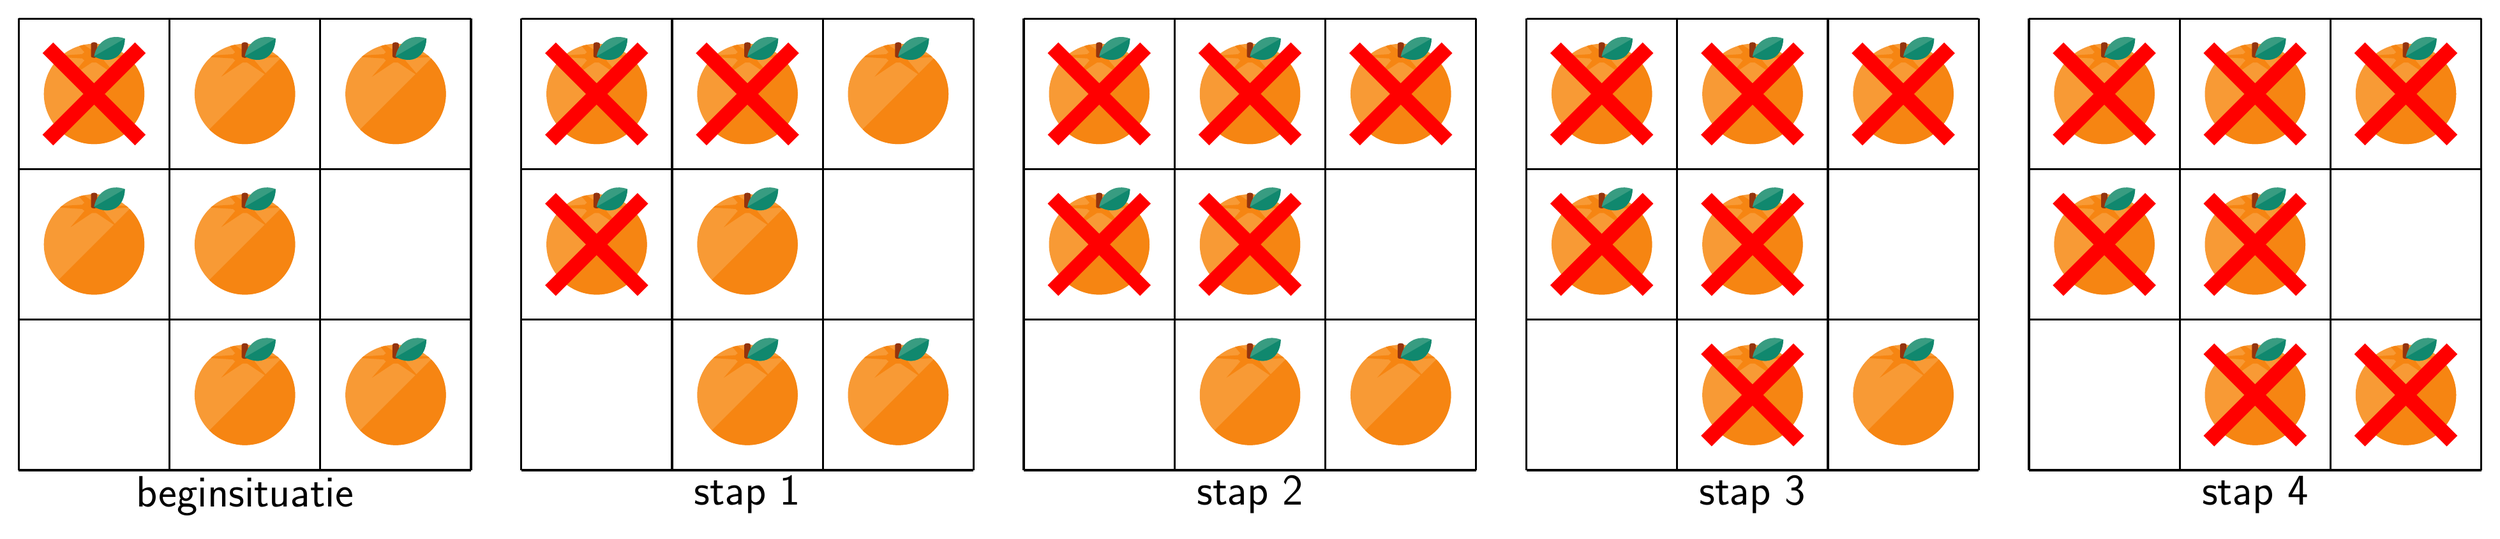
\begin{tikzpicture}[color=black]
		\begin{scope}
			\draw[very thick] (0,0) grid[step=3] (9,9);
			\draw (1.5,7.5) pic {orange};
			\draw (1.5,7.5) pic {cross=1.3cm};
			\draw (1.5,4.5) pic {orange};
			
			\draw (4.5,7.5) pic {orange};
			\draw (4.5,4.5) pic {orange};
			\draw (4.5,1.5) pic {orange};
			
			\draw (7.5,7.5) pic {orange};
			\draw (7.5,1.5) pic {orange};
			\draw (4.5,0) node [below] {\Huge \sf beginsituatie}; 
		\end{scope}
	
		\begin{scope}[xshift=10cm]
			\draw[very thick] (0,0) grid[step=3] (9,9);
			\draw (1.5,7.5) pic {orange};
			\draw (1.5,7.5) pic {cross=1.3cm};
			\draw (1.5,4.5) pic {orange};
			\draw (1.5,4.5) pic {cross=1.3cm};
			
			\draw (4.5,7.5) pic {orange};
			\draw (4.5,7.5) pic {cross=1.3cm};
			\draw (4.5,4.5) pic {orange};
			\draw (4.5,1.5) pic {orange};
			
			\draw (7.5,7.5) pic {orange};
			\draw (7.5,1.5) pic {orange};
			\draw (4.5,0) node [below] {\Huge \sf stap 1}; 
		\end{scope}
		
		\begin{scope}[xshift=20cm]
			\draw[very thick] (0,0) grid[step=3] (9,9);
			\draw (1.5,7.5) pic {orange};
			\draw (1.5,7.5) pic {cross=1.3cm};
			\draw (1.5,4.5) pic {orange};
			\draw (1.5,4.5) pic {cross=1.3cm};
			
			\draw (4.5,7.5) pic {orange};
			\draw (4.5,7.5) pic {cross=1.3cm};
			\draw (4.5,4.5) pic {orange};
			\draw (4.5,4.5) pic {cross=1.3cm};
			\draw (4.5,1.5) pic {orange};
			
			\draw (7.5,7.5) pic {orange};
			\draw (7.5,7.5) pic {cross=1.3cm};
			\draw (7.5,1.5) pic {orange};
			\draw (4.5,0) node [below] {\Huge \sf stap 2}; 
		\end{scope}
	
		\begin{scope}[xshift=30cm]
			\draw[very thick] (0,0) grid[step=3] (9,9);
			\draw (1.5,7.5) pic {orange};
			\draw (1.5,7.5) pic {cross=1.3cm};
			\draw (1.5,4.5) pic {orange};
			\draw (1.5,4.5) pic {cross=1.3cm};
			
			\draw (4.5,7.5) pic {orange};
			\draw (4.5,7.5) pic {cross=1.3cm};
			\draw (4.5,4.5) pic {orange};
			\draw (4.5,4.5) pic {cross=1.3cm};
			\draw (4.5,1.5) pic {orange};
			\draw (4.5,1.5) pic {cross=1.3cm};
			
			\draw (7.5,7.5) pic {orange};
			\draw (7.5,7.5) pic {cross=1.3cm};
			\draw (7.5,1.5) pic {orange};
			\draw (4.5,0) node [below] {\Huge \sf stap 3}; 
		\end{scope}
	
		\begin{scope}[xshift=40cm]
			\draw[very thick] (0,0) grid[step=3] (9,9);
			\draw (1.5,7.5) pic {orange};
			\draw (1.5,7.5) pic {cross=1.3cm};
			\draw (1.5,4.5) pic {orange};
			\draw (1.5,4.5) pic {cross=1.3cm};
			
			\draw (4.5,7.5) pic {orange};
			\draw (4.5,7.5) pic {cross=1.3cm};
			\draw (4.5,4.5) pic {orange};
			\draw (4.5,4.5) pic {cross=1.3cm};
			\draw (4.5,1.5) pic {orange};
			\draw (4.5,1.5) pic {cross=1.3cm};
			
			\draw (7.5,7.5) pic {orange};
			\draw (7.5,7.5) pic {cross=1.3cm};
			\draw (7.5,1.5) pic {orange};
			\draw (7.5,1.5) pic {cross=1.3cm};
			\draw (4.5,0) node [below] {\Huge \sf stap 4}; 
		\end{scope}
		
	\end{tikzpicture}
\end{document}